%整体思路: 
%1. 在特征方面,引入了aging的特征
%2. 在训练模型的时候,引入了smoteboost的方法来采样



\documentclass{acm_proc_article-sp}

\usepackage{algorithm} %format of the algorithm
\usepackage{algorithmic} %format of the algorithm
\usepackage{multirow} %multirow for format of table
\usepackage{amsmath}
\usepackage{xcolor}
\DeclareMathOperator*{\argmin}{argmin}         %argmin或argmax公式的排版 

\renewcommand{\algorithmicrequire}{\textbf{Input:}}   %Use Input in the format of Algorithm 
\renewcommand{\algorithmicensure}{\textbf{Output:}}  %UseOutput in the format of Algorithm 


%
\begin{document}


%
\title {Leveraging  Aging Theory in Multi-news Timeline Summarization} 

\author{
% 1st. author
\alignauthor
Chen Jie\\
     \affaddr{Beijing Institute of Technology}\\
       \affaddr{ 5 South Zhongguancun Street }\\
       \affaddr{Haidian District, Beijing}\\
       \email{sonyfe25cp@gmail.com}
% 2nd. author
\alignauthor
Zhendong Niu\\
         \affaddr{Beijing Institute of Technology}\\
       \affaddr{ 5 South Zhongguancun Street }\\
       \affaddr{Haidian District, Beijing}\\
       \email{zniu@bit.edu.cn}\\
}
\maketitle
\begin{abstract}

%In order to summarize multiple news about the same event, it's often helpful to follow the development progress of them.
%We present a model based on aging theory which provides an intuitive way to show the life circle of the event, complying with the habit of people understanding things.
%We summarize these news within three steps.
%First, we reduce the influence of synonyms with the LSA method for each sentence.
%Second, aging theory is introduced to represent the sentence with other four categories of features which are common used in this field. 
%Third, a classifier model is trained by SVM to recongized the summary sentence with the help of those features
%Experiment results show that our method can improve the timeline summarization significantly.

This paper focuses on the problem of news event timeline summary in Multi-Document Summarization(MDS), which aims to summarize multi-news regarding the same event in timeline.
Traditional methods to solve this problem only consider the text surface features and topic-related features, such as length of each sentence, position of the sentence in the document, number of topic words and so on.
They ignored the life circle of the news event, each event has its characteristics which are shown in the change of words distribution.
This paper proposes a new feature to describe the event based on the aging theory which focus on the life circle about the words.
Sentences and their publish date are extracted from each news report.
Then, servel pretreatment work are done to these sentences to reduce the influence of noises like synonyms.
After that, aging features and other four categories of features which are common used in this field are collected.
Finally, SVM model is used to train these features with SMOTE technology to recongized the summary sentence.
Experiment results show that our method can improve the timeline summarization significantly.

\end{abstract}

%
\section{Introduction}
%

Important facts about the news event summary are those which descripe the development progress of it.
When people create summaries, they choose the sentences which contain key words such as place, people, date and so on to form a short story about the event.
Understandably in automatic summarization as well, it's useful to use those key words to represent general facts and the important factors.

Everyday thousands of news reporting different events are published on the internet. 
There are lots of news services(e.g. Google News) have been developed to group news into events, and then produce a short summary for each event.
However, most news reports are not prepared for the progress of event, lots of duplicate messages among reports about the same event. 
#Topic-focused multi-document summarization aims to the main information from those topic-focused documents. 
Multi-news summarization aims to the main information about the event progress from these news reports.
The timeline summarization help to reorganize the order and sentences selection to get a better reading experience.

A particular challenge for multi-document summarization is how to computing the importance of each sentence, which is either depend on the words or some other latent information about the sentence.
This required effective methods to analyze the information stored in different sentences.
From the surface of different sentences, there are many synonym and polysemy words which bring lots of difficulties when computing relationships among sentences.
Latent semantic analysis (LSA) \cite{1990-Deerwester-p391-407} is introduced to find the core words in a document to avoid the influence caused by those words.
LSA is a robust unsupervised technique for deriving an implicit representation of text semantics based on observed co-occurrence of words to find semantic units of news.


Another challenge for multi-document summarization is how to deal with duplicate information among these documents about the same topic or event.
Reporters usually like to review something happened and then tell the readers what happens now. 
It's helpful for readers to know the development progress about the topic and also a solution to this challenge.
Event goes through a life cycle of birth, growth, maturity and death, and this can be reflected from special terms utilized for descripting different events experience a similar life cycle. 
Aging theory \cite{chen2003life} is a model exploited in event detection task which tracks life cycles of events using energy function. 
The energy of an event increases when the event becomes popular, and it diminishes with time. 
In intuition, it can also be used for summarization to help us find out the daily hot terms of events. 


In this paper, we generate timeline summary by considering both temporal and semantic characteristics from the news regarding the same event.
Sentences and publish time are extracted from the news articles. 
We extract the features from five aspects to represent each sentence. 
Then, classification model is built with logistic regression. 
Finally, we choose sentences from candidates to form the summary and display them with timeline, so that people can track the progress of event easily and quickly.

The remainder of this paper is organized as follows: Section 2 reviews related works on summarization and aging theory. 
We discuss our approach about how to leverage aging theory to gain sentence feature and train the logistic regression classification model in section 3. 
Experiments and discusses are described in section 4. 
Section 5 presents our conclusions and future plans.


%
\section{Related Work}

\subsection{Multi-Document Summarization}

Many summarization methods about multi-document have been developed recently. 
Generally speaking, these methods can be divided into extractive summarization or abstractive summarization.
The main idea of extractive summarization is to assign scores to different words in each sentence, then those sentences with high scores will be choosed as the summary.
While abstractive summarization usually do some information fusion\cite{barzilay1999information}, compression\cite{2002-Knight-p91-107} and reformulation\cite{mckeown1999towards} to get the summary sentences.
In this paper, we focus on the former method.

One of the most popular extractive multi-document summarization methods is MEAD\cite{2004-Radev-p919-938}, which represents each sentence with some sentence-leve features such as term frequency, sentence position, first-sentence overlap, etc. 
Wan\cite{wan2007manifold} proposed an extractive approach based on manifold-ranking about the information richness and novelty.
%Wan\cite{2008-Wan-p299-306} used markov random walk model and cluster hits model to analysis the link relationships between sentences in order to gain the important one as the summary. 
News Blaster\cite{McKeown2003} clusters news into events and apply the MultiGen system to find similar senteces and reform the pieces of sentences to create the summary.
Allan\cite{2001-Allan-p10-18} used 'usefulness', 'novelty' to represent the sentence and provide summaries of news topics. 
They aimed to deal the news stream and create the useful summary sentences.
Wong\cite{2008-Wong-p985-992} investigated co-training method by combining labeled and unlabeled data to train the model, which used four kinds of features can be categorized as surface, content, relevance and event features.

Most recently, the multi-document timeline summarization gains enough attraction from researchers and engineers.
The timeline can help readers to know the development  progress of the event.
This requires the redundancy of summary should be very low and the key properties of event should be retained. 
Lots of timeline summarization methods and applications have been developed recently. 
ETS\cite{2011-Yan-p745-754} formulated the task as an optimization  problem via iterative substitution from a set of sentences with four requirements. 
Tran\cite{tran2013leveraging} investigated five different sentence features and leveraged SVMRank to optimize the summarization task and proposed an un-biased criteria which can model timeline's characteristics.
Zhao\cite{zhao2013timeline} took social attention involved to compute the importance and capture social attention by learning users' collective interests in the form of word distributions from Twitter.
Yan\cite{Yan-2011-TGT-2145432-2145483} proposed to model trans-temporal correlations among component summaries for timelines, using inter-date and intra-date sentence dependencies.
Nedunchelian\cite{2008-Nedunchelian-p480-485} reused the MEAD and add the timestamp feature to implement their TS.
Binh Tran\cite{binh2013structured} extracted the temporal information and surface features to train the regression model for predicting the summary sentences. 
And in the same year, they\cite{binh2013predicting} proposed a framework for automatically constructing timeline summaries from web news articles. In their framework, they extracted some features for each date about articles and sentences' published time and reference time.

\subsection{Aging theory}

Different aspects are shown in different stages of each event.
An effective way to extract hot topic words is that capturing variations  in the distribution of different word terms occur in the documents regarding the event.
Therefore, tracking the terms to know what the stage of the life cycle is very important.
Aging theory has been proved effictive to track which stage of life cycle for news. 
It modes the news event's life cycle into four stages, birth, growth, decay, and death.
This four stages can be reflected by the key words' distribution.
Chen\cite{2007-Chen-p1016-1025}\cite{chen2003life} applied this to model the news event's life cycle and utilized the concept of energy to track it. 
In order to gain the summary of multi-documents of news domain, we consider aging theory is worth using to extract the feature of sentence.

%
\section{Our Approach}
%

\begin{figure}\label{process}
\centering
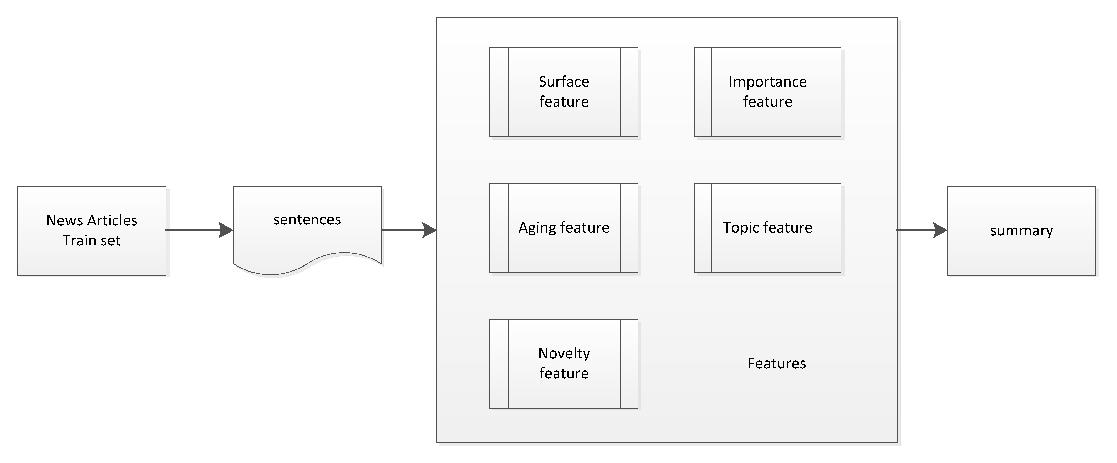
\epsfig{file=summary-process.eps, height=1in, width=3in}
\caption{The overall process of auto-summary}
\end{figure}

Figure 1 shows the overall process of our approach.
Sentences are extracted from the training set of news articles.
Then, features are computed for each sentence. 
Finally, SVM model is used to train these features with SMOTE technology to recongized the summary sentence.


\subsection{Key Concepts}

%\texttt{Topic-focused}: What we value most is an event grouped from several web news articles, such as the "the missing of the malaysia airlines plane" from BBC. These articles show us the cause, the progress and the results about the event. 
%Most of our summarrization technology's application scenario is working for TDT system. 
\texttt{Event}: News event often refers to a series of news reports about someone or something during a period of time, such as the news report about "the missing of the malaysia airlines plane". These articles form a news event which tell us the cause, the progress and the results about it. 

\texttt{Timeline Summaries:} Generally speaking, timeline is a kind of display forms for the summaries. Timeline summaries should show us the progress of this topic instand of just displaying the message according to the time sequence. Under this condition of the requirement, timeline summary of each day should describe the most important thing happened in that day.

We give the formal definition of event timeline summarization as follows:

\textit{Input}: Given a set of news articles $D=\{d_1, d_2, \dots, d_n\}$ which should cover progress of the event in the time span $T=\{t_1, t_2, \dots, t_m\}$. We segment each news into sentences and group them by the date to form sentences $S=\{s_1, s_2, \dots, s_m\}$. 

\textit{Output}: The multi-document timeline summarization should output the summaries along the date and each summary is the main idea of what occured in that day, i.e. $O=\{o_1, o_2, \dots, o_m\}$, where $o_i$ means the summary of sentences from all the sentences of that day $s_i$. 


\subsection{Sentence Feature Selection}

In order to respresent the most important thing happened in that day, the summary should consider the importance, the movelty, and contains the topic hot terms. 
%Five kinds of features are chosen as follows:
All the features used in our experiments are shown in table 1 and details as follows:

\begin{table}
\centering
\caption{List of features and their category}
\begin{tabular}{c|c}
\hline
Category & Feature\\
\hline
 & Length\\
 & the count of noun words\\
surface & the count of stop words\\
 & position in current paragraph\\
& position in the document\\
 & whether it contains person name\\
\hline
Importance & sum of LSA scores\\
 & sum/avg TFIDF\\
\hline
& the count of topic words\\
Topic & sum of topic words' weight\\
& sum of the TF top 10 words' weight  \\
\hline
Aging & the aging score of sentence\\
\hline 
Novelty & distance between current sentence and summary\\
\hline
 
\end{tabular}
\end{table}

\texttt{Surface feature}: This contains features computed by basic statistics, such as the length of sentence, the counts of noun words and stop words, the position in this document and paragraph, and whether it contains person name or not. %$Weight_{surface} = \{Length_{sentence}, Count_{nourms}, Count_{stopwords}, Position_{indocument}, Position_{inparagrph}, Boolean_{containspersonname}\}$

\texttt{Importance feature}: This feature aims to respesent the importance of the sentence. The weight of sentence is computed through linear combination of term weights with latent semantic analysis. The function is 
\begin{equation}
Weight_{importance} = \sum_{w \in sentence}TF_w * LSA_w
\end{equation}
where $TF_w$ is the term frequency of word $w$ and $LSA_w$ is the weight of word in the LSA results.

\texttt{Aging feature}: We use this feature to show the life cycle of the sentence. The frequency of a word will change as event going on, so we use the association between word  and time interval  to indicate its energy which is defined as follows:
\begin{equation}
  E_{w,t} =F(F^{-1}E_{w,t-1}+\alpha\cdot\chi^2_{w,t})
\end{equation}
where $E_{w,t}$ is the energy of word $w$  in time interval $t$ , $E_{w,t-1}$  is the energy of word $w$ in time interval $t-1$ , $\alpha$ is the transfer factor, and $\chi^2_{w,t}$  is the contribution degree of word  at the time interval $t$, which can be computed as presented in \cite{2000-Swan-p49-56}. 

However, no words descripting a special event point will retain popular forever, they will decay over time. In order to represent the word's life span realistically, we cut down the energy of word by a decay factor $\beta$ at the end of every time interval.
Once the energy value became negative, it will be replaced by zero and stop decaying.


According to the description above, if the energies of some words increase greatly, we can draw a conclusion that there is a hot event spot. So we need to calculate the variance of word energy next. Here we use standard deviation:
\begin{equation}
Var_{w,t} = \sqrt{ \frac{1}{N} \sum_{t \in period}(E_{w,t}- \overline{E_{w}})^2}
\end{equation}
where $N$ is the number of time intervals during the given period, $E_{w,t}$  is the energy of word $w$  in time interval $t$ , $\overline{E_{w}}$  is the average energy during the period, and $Var_{w,t}$  is the variance of $w$ .
Then each word will be assigned a new weight besides the traditional TF*IDF which can be defined as:
 \begin{equation}
Weight_{aging}=\sum_{w \in sentence_i}TF*LSA_{w} + \mu \cdot Var_{w}
\end{equation}
This kind of new weight can help us identify both central and hot information, so people can capture the main line and new changes of events simultaneously.

\texttt{Topic feature}: Each topic contains lots of sentences, that is, each sentence contribute some information to the whole set to express the topic. In this study, we use the link analysis to compute the latent semantic between sentences. First, topic terms and topic elements can be found through the word frequency analysis. Then, the similarity among sentences are computed with the cosine function to construct the event map. Last, pageRank algorithm is used to assigin the weight to each node in this map. We treat the pageRank value as the topic feature of the sentence. The function is :
\begin{equation}
Weight_{topic} = PageRank(sentence_i)
\end{equation}

\texttt{Novelty feature}: In order to avoid some sentences with the same meanings be selected as the summary, the novelty of sentence is important. 
The novelty value is computed by the distance with the summary of last time span. 
The larger the distance, the more the novelty this sentence. 
In our research, we use the Jaccard similarity to gain this value. The function is :
\begin{equation}
Weight_{novelty} = 1 - Jaccard(sentence_i, summary_{ex})
\end{equation}
where $summary_{ex}$ is the summary sentence in the last time span.



\subsection{Model Training}

In the case of annotation data, we considered this summarization task as a classification problem. The positive data is sentences labeled as summary sentences, otherwise is negative. 

However, in each document only a few sentences will be labled as the summarization sentence, that is, the dataset is imbalanced. 
When we create a classifier over such an imblanced dataset, the classifier will perfer the majority side \cite{chawla2003smoteboost}.
In order to impove the precision of minority class, we used SMOTEBoost\cite{chawla2003smoteboost} method to sampling datas for training the classification model. 
This method combines SMOTE \cite{chawla2011smote} and boost technology and has been proved effective for imbalanced data set. 


%
\section{Experiments}
%

\subsection{Datasets and Design}

Since 2001, the US National Institute of Standards and Technology (NIST) has organized large-scale shared tasks for automatic text summarization within the Document Understanding Conference\footnote{http://duc.nist.gov/} (DUC) and the Summarization track at the Text Analysis Conference\footnote{http://www.nist.gov/tac/} (TAC).
%There are so many datasets available for the summarization task, 
We choose one generic summarization and one guided summarization dataset to test our approach from these datasets.

DUC-2002 dataset is used for generic summarization task in 2002.
This dataset consist of 59 document sets, each in two formats - one with just the original TREC tagging, and one with rough sentence tagging added.
Each document set contains around 12 documents from different day about the same event.
Each event is also provided about 6 labled summary sentences with the limit of 200 words.
We also set this words limit to our experiments.

TAC-2010 dataset is used for guided summarization task.
This task aims to encourage summarization systems to make a deeper linguistic (semantic) analysis of the source documents instead of relying only on document word frequencies to select important concepts and create the summary covered the predefined category.
This dataset contains 906 documents around 46 topics from the New York Times, the Associated Press, the Xinhua News Agency newswires, and the Washington Post News Service.
Each topic has two sets of documents, A and B, each containing 10 documents.
The difference is that documents in B were published later than A.
It's also an update summarization task, since it's required to create an 100 words updated summarization about documents in B.
This dataset is good for the timeline summarization, cause the summary should contains the important facts about the predefined category and show the update information.
We relabeled the summary sentences based on the results from NIST in order to adapt the timeline  summarization.


\subsection{Baselines}
We start our experiment with some preprocessings like indexing, filtering out the stop words and segmenting news documents into sentences. Then we perform our method to the data set and generate a timeline for each event we choosing. We implement some widely used multi-document summarization methods as the baselines.

$Random$ The strategy for random method is that one sentence will be choosed as the summary sentence randomly from the whole document.

$MEAD\footnote{http://www.summarization.com/mead}$ is a famous multi-document summarization tools which extracts summary sentence based on centroid value, positional value and first-sentence overlap.

$Cluster$ considers that there are different themes in an event, so it devide clusters similar sentences together into different clusters and then selects one representative sentence from each main cluster.

$Allan$ is a similar timeline system from different aspects, which dividing sentences into on-event and off-event while ranking them with useful and novelty.

$Wong$ combined the supervised and semi-supervised learning and used co-training method to train the labeled data and unlabeled data. 

$L2RTS$ considered the summary task as optimistic task and  leveaged the SVMRank to gain the summary.

\subsection{Evaluation metric}

Here we use ROUGE toolkit \cite{2004-Lin-p74-81} , which is officially applied by DUC for document summarization performance evaluation, to evaluate the experimental results and compare these algorithms with each other. 
It's a recall based measure which compute unigram or bigram words matching between the auto-summarization summary and human labeled summary sentences.
All the summaries were truncated to the words limit size without removing the stop words.

\subsection{Results}

We use LibSVM\footnote{http://www.csie.ntu.edu.tw/~cjlin/libsvm/} to train the classification model.
The model in our approach 1 is trained without SMOTEBoost, while the approach 2 is trained with re-sampling technology of SMOTEBoost.
Rouge-1 and Rouge-2 are used to measure the performance about recall on both datasets. Results are shown in Table 2 and Table 3.
Precision measures the percentage of labeled summary sentences among all the summary sentences created by the classifier.


\begin{table}
\caption{Performance on DUC-2002 dataset}
\centering
\begin{tabular}{llll}
\hline\noalign{\smallskip}
Method   &  Precision    & Rouge-1  				& Rouge-2 \\
\noalign{\smallskip}
\hline
\noalign{\smallskip}
Random & 0.023 			& 		0.024 			&  0.013 \\
MEAD    &	0.121			& 		0.105	 			&	0.048					 				\\
Cluster	&	0.075			&		0.061				&	0.018					 				\\
Allan		&	0.077			&		0.061				&	0.021						 			\\
Wong		&	0.144			&		0.245				&	0.089									\\
L2RTS	&	0.211			&		0.276				&	0.105						 			\\
Our approach 1	&	\textbf{0.204}	&		\textbf{0.273}				&	\textbf{0.103}	 \\
Our approach 2	&	\textbf{0.221}	&		\textbf{0.279}				&	\textbf{0.110}	 \\
\hline
\end{tabular}
\end{table}

\texttt{Generic summarization} From Table 2, it can be seen that our approach 2 using svm and SMOTEBoost obtains the best results, followed by the $L2RTS$ then the approach 1 then $Wong$ and $MEAD$. 
There is no surprise that Random provides the worst results. 
The approach 2 performances better than approach 1 is well understanded, since the resampling can gain more training samples which enhance the classifier.
The $Allan$'s approach is similar timeline, but the results are not good due to the fact that only useful and novelty features are not enough to maintain the information of sentence. 
The $Cluster$ method's bad performance is due to the random selecting strategy from the cluster center.
$Wong$'s method combined the supervised and semi-supervised learning which make it hard to turning the parameters.
The $L2RTS$ method it better than Wong since the SVM-rank can put the preference information to the training progress.
Our approach performs better than $L2RTS$ in this experiment. This is due to the new features about aging and the training tricks about SMOTE which help the classifier to get better hyperplane.


\begin{table}
\caption{Performance on TAC-2010 dataset }
\centering
\begin{tabular}{lllll}
\hline\noalign{\smallskip}
Method   &  Precision   & Rouge-1  &Rouge-2  \\
\noalign{\smallskip}
\hline
\noalign{\smallskip}
Random &  0.037           &      0.029                &  0.017									\\
MEAD    &	0.129			& 		0.076	 			&	0.028					 				\\
Cluster	&	0.057			&		0.045				&	0.025				 				     \\
Allan		&	0.143			&		0.083				&	0.032						 			\\
Wong		&	0.214			&		0.185				&	0.073									\\
L2RTS	&	0.221			&		0.290				&	\textbf{0.124}					 	\\
Our approach 1	&	\textbf{0.211}	&	\textbf{0.279}				&	0.102		          \\
Our approach 2	&	\textbf{0.233}	&	\textbf{0.291}				&	0.121		          \\
\hline
\end{tabular}
\end{table}

\texttt{Guided summarization} Table 3 shows the results on the TAC-2010 dataset.
In this experiment, the $L2RTS$ performs bettern than our approach on the Rouge-2.
This is due to the preference information, that is, the average number of sentences in each document of this dataset is bigger than DUC-2002, which produce more information.
The $Allan$ method performs better than $MEAD$.
The reason is that events in this dataset have more than 20 documents, which provide enough information about useful and novelty compared to the previous dataset.

From this two experiments, we can get the information that summarization methods based on machine learning are performance better than others. 
The result of $MEAD$ are better than $Cluster$, mainly because this method use some surface feature.
The $Cluster$ method is the worst in our experiments, since this method cluster the same meaning sentences and choose one from cluster randomly. 
The $Allan$ method does not perform stable, that it will depend on the amount of documents and the content of each sentence. 
Our method 2 performed better than $Wong$ and $L2RTS$ on precision and Rouge-1 metric which mainly due to  SMOTE method and the new feature about aging. 
The SMOTE technology make the minorty class can be classified better and this is proved in our experiments.
But when testing in Rouge-2, the $L2RTS$ wins the match, because the SVMRanking can obtain a better classification model with enough perference information, but the complexity of algorithm is also high.

%
\section{Conclusion and Future}
%

In this paper, we present a novel approach of which involved aging theory and SMOTEBoost to timeline summarization. In our approach, we firstly construct features of each sentence, which contains surface feature, importance feature, aging feature, novelty feature and topic feature. Then we treate the multi-document summarization task as pair-wise classification task and generate the training data. At last SMOTEBoost is used to train the model combined with SVM. Experiment results show that our approach performs better compared with other widely used methods.

In the future, we will identify semantic units using other methods since $LSA$ can process synonym but is unable to handle polysemy. And we will also extend our approach to short text such as microblogs and comments.

%Acknowledge%
%\section{Acknowledgements}
%something and somebody should be thanks...



%\bibliographystyle{splncs}
\bibliographystyle{abbrv}
\bibliography{../../bib/text_summary.bib}



\end{document}
